\section{Principles of Serial Communication}
%TODO Definition von Baudrate, Bitrate, Even&Odd Parity und noch überarbeiten
\begin{multicols}{2}
	\textbf{Baud-Rate}\\
	$\frac{1}{t_{bit}}=Baud-Rate [bit/s]$\\
	\textbf{Bitrate}\\
\end{multicols}
\subsection{Data Communication Fundamentals}
	\subsubsection{Serial Data Channels}
	\begin{itemize}
		\item RX: Receiver, TX:Transmitter
		\item Main form of Communications today
		\item Broad variaton of Protocols and Formats
		\item Bits are transmitted and received one after another
		\item longer time for sending bits $n\cdot t_{bit}$
		\item Single Ended Link: Two Wires (Link, GND)
		\item Differential Link Channel: Two Wires with Voltage Difference
		\item USB, RS232,RS485, Bluetooth, Ethernet, I2C, SATA...
	\end{itemize}
\subsubsection{Parallel Data Channels}
	\begin{itemize}
		\item n Bits are transferred simultaneously in parallel
		\item needs for every bit one wire (costs!)
	\end{itemize}
	
\subsection{Types of Serial Communications}
\subsubsection{Direction of Communications}
\begin{tabular}{lll}
	\textbf{Simplex}&\textbf{Half-Duplex} &\textbf{Duplex}\\
	Unidirectional Link&  One Bidirectional Link& Two separate Bidirectional Link\\
	Only one Direction & both Directions & both Directions\\
	No ACK of Data & one Direction at one Time & Simultaneous Communication\\
	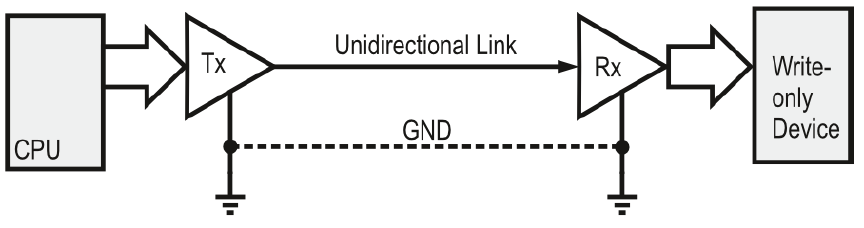
\includegraphics[width=6cm]{images/simplex.png}& 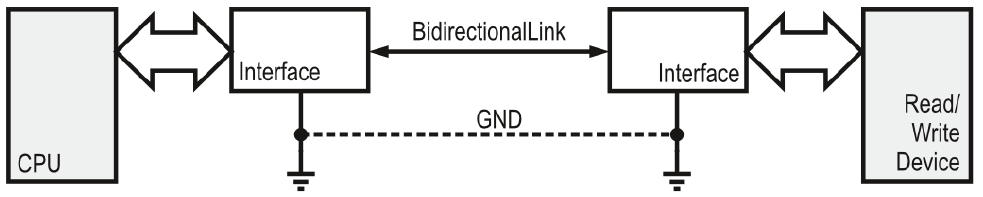
\includegraphics[width=6cm]{images/half_duplex.png}&
	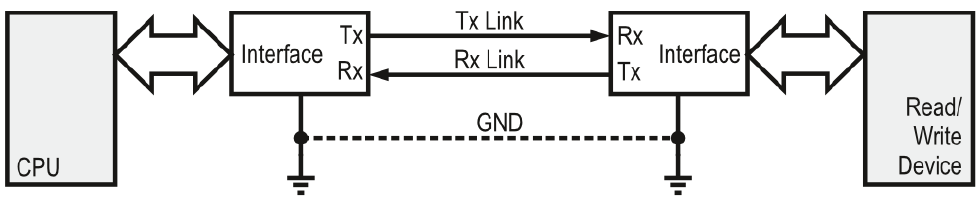
\includegraphics[width=6cm]{images/duplex.png}\\
\end{tabular}	
\subsubsection{Topologies}
\begin{itemize}
	\item Point-to-Point
	\item Bus
	\item Line
	\item Star
	\item ring
\end{itemize}	
\clearpage
\pagebreak
\subsection{Asynchronous Serial Communication}
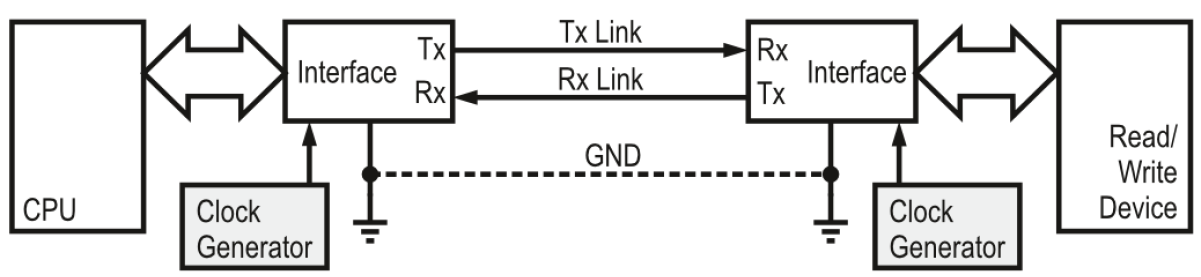
\includegraphics[width=8cm]{images/asyn.png}
\begin{itemize}
	\item Synchronous Communication the clock is send with data
	\item Independent Clock at both Ends	
	\item Clocks must be synchronized regularly
	\item Each Package consiist of Header (begin Data), Body (Data), Footer (delimits the Packet)
	\item Same Data rate at both Ends
	\item Falling Edge of Startbit starts Sampling at RX
	\item Receiver Samples in the middle of each Bit
	\item If RX runs too fast then ends in incorrect Datagram
	\item Bad Rate Erros of $2\% to 4\%$ are tolerable
\end{itemize}
\subsubsection{Error Detection Mechanism}
\begin{itemize}
	\item Even Parity:
	\item Odd Parity:
	\item Parity Bit:can be configured to Even, Odd, None, Mark, Space
	\item Stop Bit: marks the End of the Transmission, always Mark
\end{itemize}
\subsubsection{UART (Universal Asynchronous Receiver Transmitter)}
\begin{minipage}{10cm}
	\begin{itemize}
		\item convert Data from Parallel to Serial and viceversa
		\item allow the CPU to communicate through the Serial Channel
		\item USART: supports Asynchronous and Synchronous Communications Channels in one single Serial Interface Module
	\end{itemize}
\end{minipage}
\begin{minipage}{9cm}
	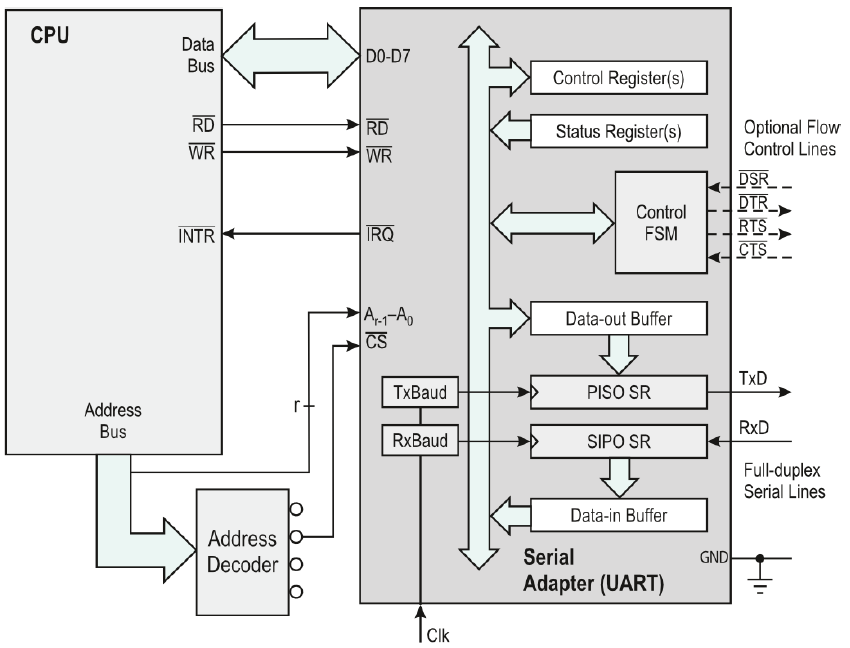
\includegraphics[width=9cm]{images/uart.png}
\end{minipage}


\subsubsection{RS-232}
\subsubsection{RS-485}
\subsubsection{USB}
\begin{multicols}{2}
	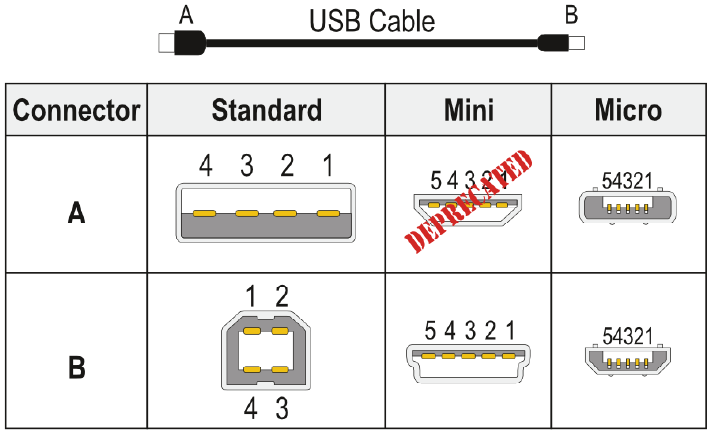
\includegraphics[width=8cm]{images/usb_jacks.png}\\
	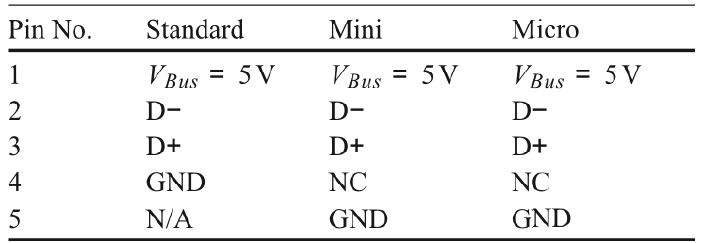
\includegraphics[width=8cm]{images/usb_voltage.png}\\
\end{multicols}
\clearpage
\pagebreak